%%%%%%%%%%%%%%%%%%%%%%%%%%%%%%%%%%%%%%%%%%%%%%%%%%%%%%%%%%%%
% Document settings
\documentclass{ACGSeminar}

%%%%%%%%%%%%%%%%%%%%%%%%%%%%%%%%%%%%%%%%%%%%%%%%%%%%%%%%%%%%
% Own Packages
\usepackage{amsmath}

%%%%%%%%%%%%%%%%%%%%%%%%%%%%%%%%%%%%%%%%%%%%%%%%%%%%%%%%%%%%
% Own Definitions
\newcommand{\comment}[1]{}


%%%%%%%%%%%%%%%%%%%%%%%%%%%%%%%%%%%%%%%%%%%%%%%%%%%%%%%%%%%%
% BibTex
\bibliography{references}

%%%%%%%%%%%%%%%%%%%%%%%%%%%%%
% Hyphenations here
%%%%%%%%%%%%%%%%%%%%%%%%%%%%%
\hyphenation{Sa-tan-arch-aeo-li-deal-co-hell-ish}


%%%%%%%%%%%%%%%%%%%%%%%%%%%%%
% Title, Author, etc.

\begin{document}

\title{Instant Field-Aligned Meshes}

\author{Til Mohr}


\maketitle

%%%%%%%%%%%%%%%%%%%%%%%%%%%%%%%%%%%%%%%%%%%%%%%%%%%%%%%%%%%%
% Abstract

\begin{abstract}
Remeshing geometries into uniform models is an essential preceding task to many geometry processing algorithms. This paper will examine the instant field-aligned remeshing algorithm presented by Jakob et al. Doing so, this article will first introduce all key concepts used in the algorithm, and will later on present,
how the authors combine these concepts to form their remeshing algorithm. This approach stands out since uses locally optimized orientation- and position-fields to compute an isotropic triangular or quad-dominant mesh that is globally aligned with a direction field. Since it accomplishes goals from global remeshing using local optimizations, the method is quite simple complexity-wise and can produce high-quality meshes in no time. To compare to this approach, this paper will also take a closer look at other meshing algorithms and will analyze the performance and quality differences in the resulting meshes.
\end{abstract}

\keywords{remeshing, triangulation, quadrangulation}
\tableofcontents

\newpage

%%%%%%%%%%%%%%%%%%%%%%%%%%%%%%%%%%%%%%%%%%%%%%%%%%%%%%%%%%%%
% Introduction
\label{cha:introduction}
\section{Introduction}
\begin{itemize}
	\item	Why remeshing? $\rightarrow$ Many geometry processing algorithms (smoothing, compression, ...) benefit from isotropic remeshing \cite{surazhsky2003isotropic}. (This is where the paper fits amongst the other papers of the seminar)
\end{itemize}

%%%%%%%%%%%%%%%%%%%%%%%%%%%%%%%%%%%%%%%%%%%%%%%%%%%%%%%%%%%%
% Background
\section{Background and Terminology}
To fully understand how the algorithm works, we first need to understand some key concepts and techniques. This also helps us to distinguish this approach from other remeshing algorithms.

\subsection{Polygonal meshes}
In computer graphics, there are many possible ways to represent surfaces of digital geometries, such as parametric surfaces, subdivision surfaces, and polygonal meshes. In this paper, we only focus on the latter.\bigskip

A polygonal mesh is a set of polygonal faces, each representing a 2D surface embedded in 3D. Each face consists of a vertex, a 3D point, and edges connecting these vertices. The idea behind polygonal meshes is \textit{cell decomposition}: a complex digital geometry is composed of numerous simple polygonal cells \cite{bommes2013quad}. This allows for performance optimization and reduction of complexity since as an example geometrical formulas on simple polygons are often already predefined. It is very desirable to reduce the number of vertices of each polygonal face to remove complexity. Therefore, polygonal meshes with only very few vertices per face are dominant in computer graphics and geometry processing. The most common categories are triangle meshes and quad meshes. The best type of polygon for a mesh depends on its application.\bigskip

\textbf{Quad meshes} are meshes, where each cell is a quadrilateral. They have a tensor product structure, which is beneficial to many applications such as spline fitting. Because quad meshes have this mathematical benefit, many algorithms are better suited for quad meshes than triangle meshes. Hence they play a major role in computer graphics and geometry processing \cite{bommes2013quad, chen2019quadrilateral}.

Although the quality of a quad mesh isn't specifically defined, there are some indices of a high-quality quad mesh - depending on the application -, such as flat and square faces, and vertices of valency 4. Creating a high-quality pure-quad mesh is a quite challenging task, however. When the geometry's surface has boundaries and curvatures forcing the meshes grid, which is created by square faces, to conform to them, singularities are unavoidable. A \textbf{Singularity} in a mesh is a vertex with irregular valency, a regular valency in a quad mesh, of course, being 4 \cite{fogg2017simple,fogg2018singularities}.

\begin{figure}[htb!]
	\begin{centering}
		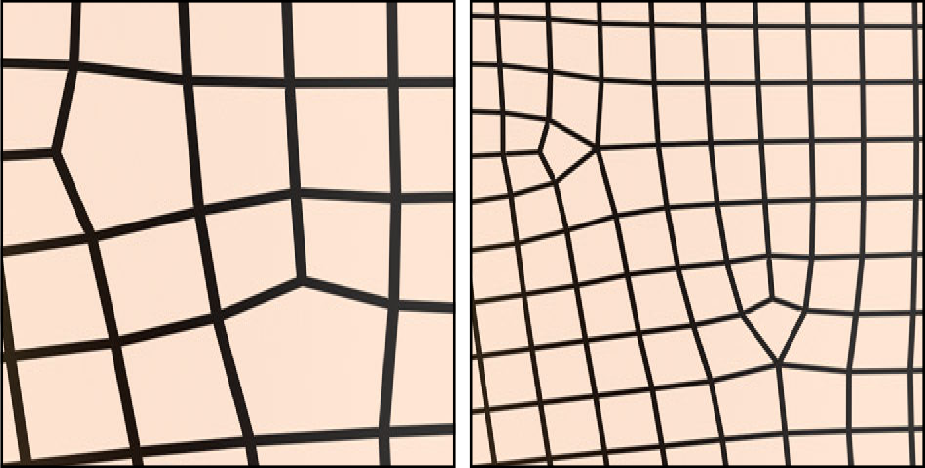
\includegraphics[width=9cm]{img/Singularities.png}\par
	\end{centering}
	\caption{Singularities create pentagons or triangles in quad-dominant mesh \textit{(left)}. Can be transformed into a pure-quad mesh through a subdivision step \textit(right). \cite{jakob2015instant}}
	\label{fig:singularities}
\end{figure}

Because handling these singularities is complicated on its own, oftentimes meshing algorithms resort to quad-dominant meshes. \textbf{Quad-dominant meshes} are meshes, where the majority of faces are quadrilaterals, with some being triangles or pentagons. A quad-dominant mesh can however be converted into a pure-quad mesh through a subdivision step \cite{jakob2015instant}.\bigskip

When a tensor product structure is not needed, often \textbf{triangle meshes} are used because of the reduced number of vertices in comparison to quad meshes, resulting in simplified geometrical calculations. Additionally, triangle meshes are always and easily computation-wise composed purely of triangular faces, that are of course by nature always flat. Because of these benefits, modelling a triangle mesh from data or even scratch can be a lot easier than modelling quad meshes. As an example, 3D scans produce triangle meshes, although often very nonuniform.\bigskip

\begin{figure}[htb!]
	\begin{centering}
		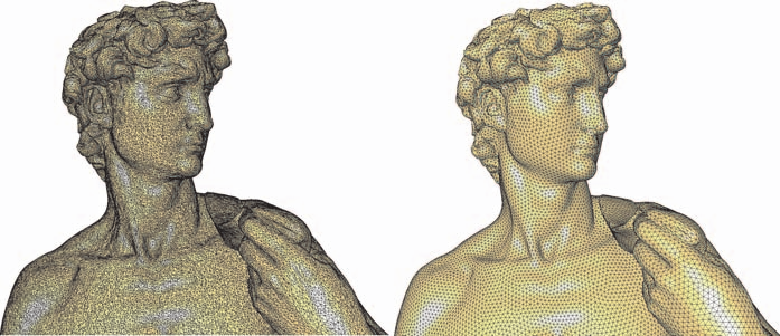
\includegraphics[width=9cm]{img/Uniform-Mesh.png}\par
	\end{centering}
	\caption{Nonuniform mesh \textit{(left)} and its uniform counterpart after uniform remeshing \textit{(right)} \cite{alliez2008recent}.}
	\label{fig:uniform-mesh}
\end{figure}

A mesh is \textbf{uniform} when its faces are as "uniform" as possible. This means the faces are of the same size and of the same shape. Additionally, \textbf{isotropy} is an important property of meshes. A mesh is isotropic, when its faces are aligned in certain directions. So combined, an uniform and isotropic mesh consists of equilateral triangles in triangle meshes or squares in quad meshes \cite{alliez2003isotropic,surazhsky2003isotropic}. While modelling triangle meshes, it is not uncommon that the resulting meshes are very nonuniform and have many redundant faces. Algorithms performing on triangle meshes can heavily struggle under such conditions. Therefore, it is quite beneficial to simplify such meshes into uniform replicas while also minimizing face count, without losing the shape of the original geometry (figure \ref{fig:uniform-mesh}).


\subsection{Global and local remeshing}
As already stated, many meshes are created through automatic processes like 3D scanning, which do often result into low quality meshes. For many geometry processing algorithms these meshes are dissatisfactory and will result in performance and quality losses. So there is a need to reduce the complexity of these meshes, to improve their quality, and sometimes even transform them into an entirely different type of mesh. This process is called \textbf{remeshing} \cite{alliez2008recent}.\bigskip

Although there are several central issues to all remeshing techniques, one especially complex one is to find the corresponding location of a new vertex on the input mesh. This is where all remeshing techniques are categorized into two classes: Global remeshing and local remeshing.\bigskip

\textbf{Global remeshing} tackles the correspondence problem through mesh parameterization. Mesh parameterization is the process of finding a parametric equation of the meshes surface. Since the input and output mesh should share the same surface, finding the corresponding location of a new vertex on the input mesh is quite uncomplicated, given that the parametric equation is known. Therein lies the main drawback with this global approach: Determining a parametric equation of a surface is a challenge, which can be quite computationally expensive and suffer from inaccuracy amongst other issues. However, if the input mesh was successfully parameterized, a high quality mesh can easily be produced \cite{jakob2015instant,alliez2008recent}.

To sum up, global remeshing techniques suffer from efficiency and simplicity, however can yield high quality meshes. A few great approaches to this technique are the "Mixed-Integer Quadrangulation" algorithm by Bommes et al. and "Periodic Global Parameterization" by Alliez et al.\bigskip

On the other hand there are \textbf{local remeshing} techniques. These algorithms do without mesh parameterization and rather work directly on the surface itself. Also, instead of creating an entirely new output mesh, local remeshing algorithms locally modify the input mesh itself, such as adding, relocating, and removing vertices. During these modifications, the vertices are always forced to rest on the surface or rather mesh. \textbf{2D 3D?!?!?!??! TODO !=!=!=!==!=!=}. This process is highly scalable, robust and simple. However, since the process is limited to only local information at a time, it is limited. Hence, local remeshing techniques usually tend to be of lower quality than global remeshing techniques, and also introduce mesh singularities due to its locality \cite{jakob2015instant,alliez2008recent}. \textbf{ANOTHER PAPER=!=!=!}


\subsection{$N$-RoSy fields}\label{rosy}
In geometry a $N$-way rotational symmetry is a property a shape has when it is invariant under rotations of a multiple of $\frac{2\pi}{N}$ around a point or an axis in 2D or 3D respectively \cite{palacios2007rotational}. One can think of these symmetries as vector fields, where each point is associated with $N$ vectors, each pointing in one direction where the symmetry repeats (figure \ref{fig:n-rosy-singularities}). Hence, we also call these symmetries $N$-way rotational symmetry fields (\textbf{$N$-RoSy fields}) \cite{panozzo2012fields}.

\begin{figure}[htb!]
	\begin{centering}
		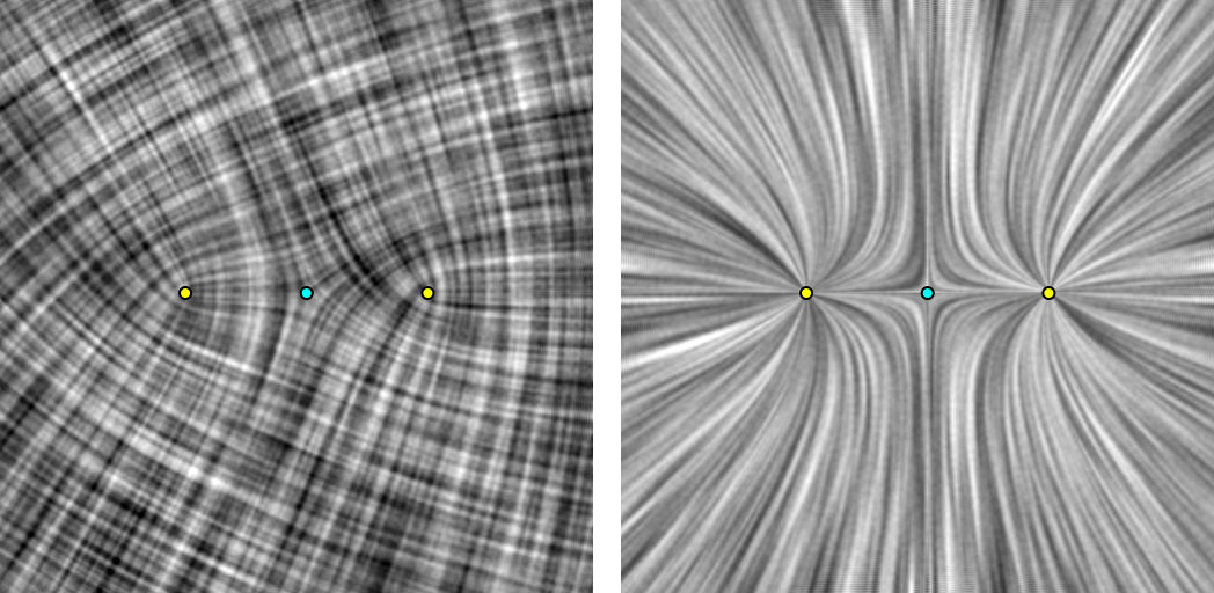
\includegraphics[width=9cm]{img/n-Rosy-Singularity.png}\par
	\end{centering}
	\caption{A comparison between a $4$-RoSy field \textit{(left)} and its vector field \textit{(right)}. Notice how singularities (colored dots) are of zero value in the vector field. \cite{palacios2007rotational}}
	\label{fig:n-rosy-singularities}
\end{figure}

Symmetries also appear on geometrical surfaces, where they are often defined as isometric automorphism. We differ between two categories of symmetries:
\begin{itemize}
	\item	\textbf{Extrinsic} symmetries preserve euclidean distances
	\item	\textbf{Intrinsic} symmetries preserve geodesic distances
\end{itemize}
In practice though, geometries rarely have perfect symmetries on its entire surface. On most surfaces there are only local symmetries, and even they aren't always ideal. Thus, deviations must be tolerated \cite{panozzo2012fields}.\bigskip

As a side effect of imperfect symmetries $N$-RoSy fields introduce singularities. Note that these singularities can differ from singularities introduced in meshes. A singularity in $N$-RoSy fields is a point in the vector field, where the associated vector is equal to 0 (figure \ref{fig:n-rosy-singularities}) \cite{palacios2007rotational}. Briefly, they occur when the surface bends in a way that break the directions of the $N$-RoSy field. However, because of this property, they are also the points that control the topology of the field, and thus also the layout of the extracted mesh (figure \ref{fig:n-rosy-geometry}). The automatic generation of $N$-RoSy fields with optimal number and positions of singularities remains a major challenge. Methods attempting this generally cannot operate without introducing new singularities, which then appear as artifacts on the extracted meshes \cite{lai2009metric}.

\begin{figure}[htb!]
	\begin{centering}
		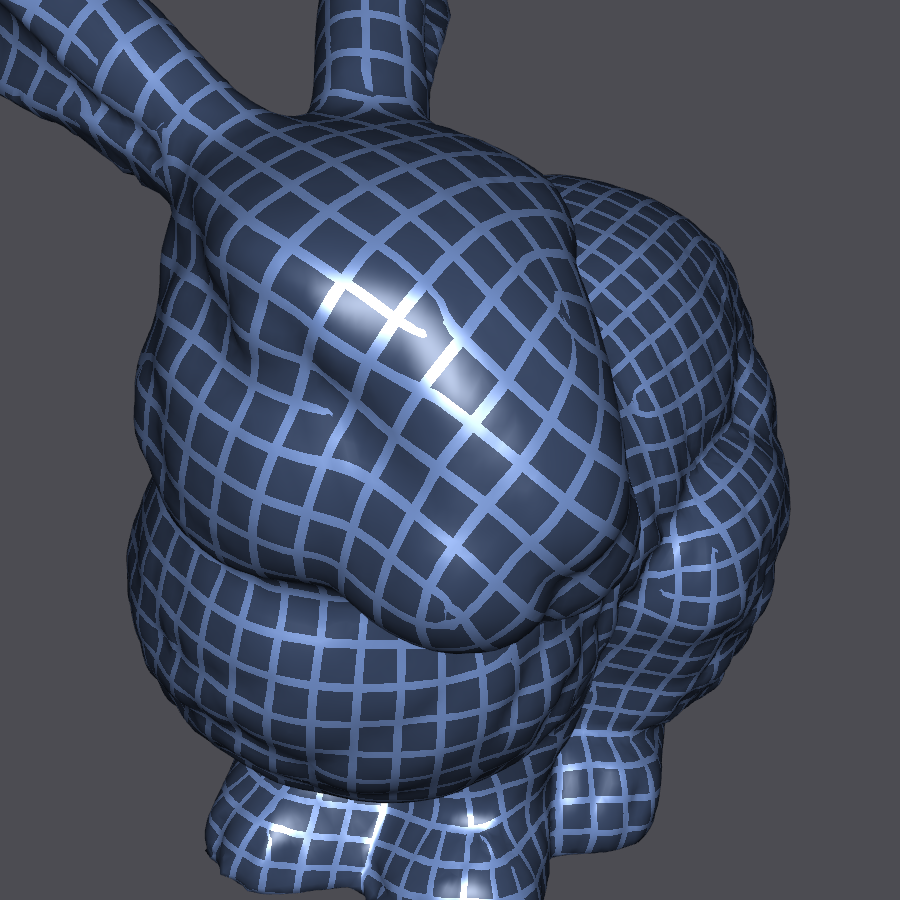
\includegraphics[width=5cm]{img/n-Rosy-Geometry.png} 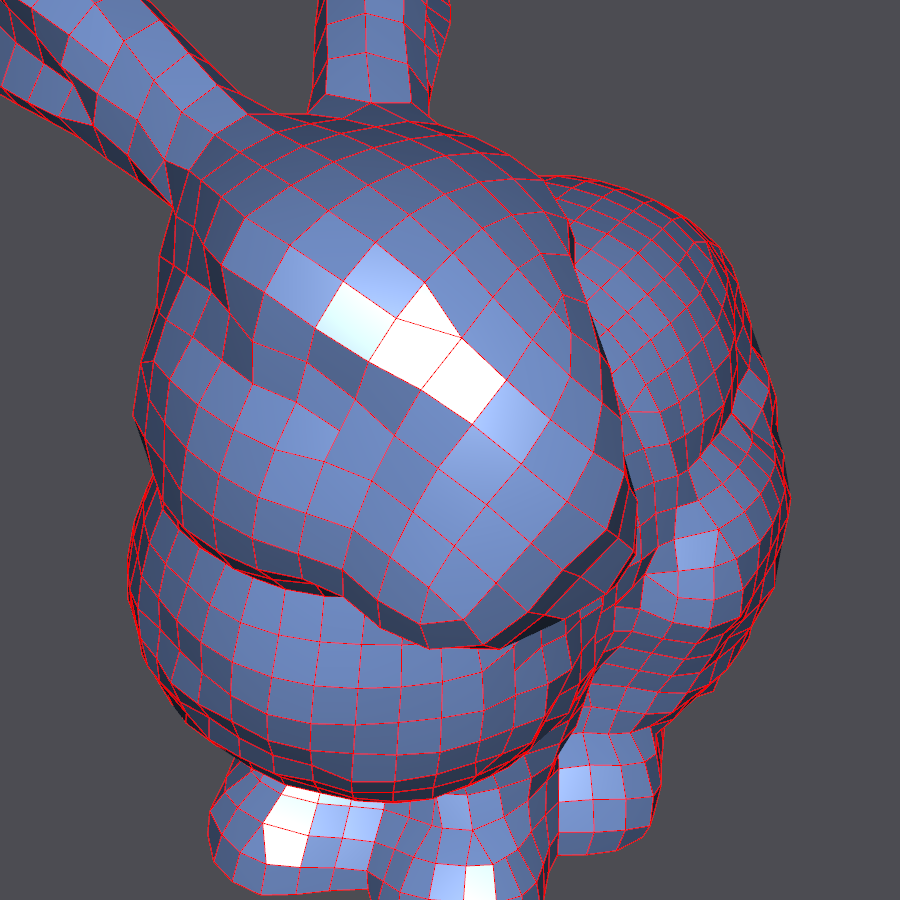
\includegraphics[width=5cm]{img/n-Rosy-Mesh.png}\par
	\end{centering}
	\caption{A $4$-RoSy field calculated from a meshes surface \textit{(left)}. Note how singularities in the $4$-RoSy field as the singularity above the eye can introduce singularities in the quad-dominant output mesh \textit{(right)}.}
	\label{fig:n-rosy-geometry}
\end{figure}



%%%%%%%%%%%%%%%%%%%%%%%%%%%%%%%%%%%%%%%%%%%%%%%%%%%%%%%%%%%%
% Related Work
\section{Related Work}\label{related_work}
\begin{itemize}
	\item	Previous remeshing approaches from \cite{jakob2015instant}: \cite{ray2006periodic,bommes2009mixed} (since they are also very similar)
	\item	\cite{marcias2015data} to compare to the data driven approach in the seminar
	\item	Focus on type of remeshing (for example local or global, triangle or quad based)
\end{itemize}

%%%%%%%%%%%%%%%%%%%%%%%%%%%%%%%%%%%%%%%%%%%%%%%%%%%%%%%%%%%%
% Main Sections
\section{Method}\label{algorithm}
The following described Instant Field-Aligned Meshes algorithm is a very simple to implement local remeshing approach.

Fundamentally, it takes a graph representation of the geometry's surface as an input and outputs either a triangle-based or a quad-dominant isotropic mesh. To create this mesh, the algorithm computes 2 $N$-RoSy fields (section \ref{rosy}) based on the input graph called orientation- and position-field respectively. In order to align the mesh globally with a direction field, the orientation- and position-field are then optimized iteratively through local smoothing operations - either intrinsically or extrinsically. The output mesh can then be extracted from both fields \cite{jakob2015instant}.

% Input
\subsection{Input representation}
As mentioned, the algorithm takes the geometry's surface represented as a graph $\mathcal{G} = (\mathcal{V}, \mathcal{E})$ for an input. Each element $i \in \mathcal{V}$ is called a vertex and represents a position $v_i \in \mathbb{R}^3$ and a normal direction $n_i \in \mathbb{R}^3$. $\mathcal{E} \subset \mathcal{V} \times \mathcal{V}$, also called the set of edges, stores neighboring vertices in the graph. Depending on the original geometrical representation, it is defined differently:
\begin{itemize}
	\item	For meshes $\mathcal{E}$ is equal to the usual set of edges in the mesh.
	\item	For point clouds $(i,j) \in \mathcal{E}$, if the vertex $i$ is in the set of $K$-nearest neighbors of $j$.
\end{itemize}
We denote the neighborhood of a vertex $i$ by $\mathcal{N}(i) = \{j \in \mathcal{V} \mid (i,j) \in \mathcal{E}\}$. Additionally, there is a weight $w_{ij}$ for each edge $(i,j) \in \mathcal{E}$. This weight affects the smoothing of the orientation- and position-field later on, and can be chosen geometry-dependent or as uniform.\bigskip

This simple input representation allows for many geometry representations to be used in this algorithm, as long as one can convert it into the described graph input format.

% Fields
\subsection{Fields}
FROM 3.1 COMPUTE SMOOTH FIELDS

\subsubsection{Orientation field}
\begin{itemize}
	\item	What for? (why is it important)
	\item	Computation (intrinsic vs extrinsic)
	\item	Singularities
\end{itemize}

\subsubsection{Position field}
\begin{itemize}
	\item	What for? (why is it important)
	\item	Computation (intrinsic vs extrinsic)
	\item	Singularities
\end{itemize}

% Multiresoluion hierarchy
\subsection{Multiresolution hierarchy}
\begin{itemize}
	\item	Problem of local minima
	\item	Solution
\end{itemize}

% Exporting
\subsection{Mesh extraction}
\cite{jakob2015instant}
\begin{itemize}
	\item	Extraction
	\item	(Editing?)
\end{itemize}

%%%%%%%%%%%%%%%%%%%%%%%%%%%%%%%%%%%%%%%%%%%%%%%%%%%%%%%%%%%%
% Results
\section{Results and Discussion}

%%%%%%%%%%%%%%%%%%%%%%%%%%%%%%%%%%%%%%%%%%%%%%%%%%%%%%%%%%%%
% Outlook
%\section{Outlook}

%%%%%%%%%%%%%%%%%%%%%%%%%%%%%%%%%%%%%%%%%%%%%%%%%%%%%%%%%%%%
% Conclusion
\section{Conclusion}
\begin{itemize}
	\item	Quite simple algorithm, but powerful
	\item	Parts can be seperated and used individually (for example you can use the orientation field generation in other algorithms as well)
	\item	Problem of many singularities needs to be dealt with
\end{itemize}

%%%%%%%%%%%%%%%%%%%%%%%%%%%%%%%%%%%%%%%%%%%%%%%%%%%%%%%%%%%%
% Bibliography
\label{cha:references}
\printbibliography

\end{document}
